
%%%%%%%%%%%%%%%%%%%%%%%%%%%%%%%%%%%%%%%%%%%%%%%%%%%%%%%%%%%%%%%%%%% 
%                                                                 %
%                           METHODS                               %
%                                                                 %
%%%%%%%%%%%%%%%%%%%%%%%%%%%%%%%%%%%%%%%%%%%%%%%%%%%%%%%%%%%%%%%%%%% 
 
% \specialhead{METHODS}
\chapter{VISUALIZATION}
\label{chapter:visualization}
In this chapter I discuss methods of visualization for the animations produced in Chapter \ref{chapter:animation}, as well as the difficulty of visualizing character animation in print format as well as video.  I present some sources of inspiration for my visualizations and motivate the need for visualizations.  I then discuss techniques I utilized to visualize my data for presentation as well as for debugging and analysis.

% talk about instpiriations here instead of prev work
\section{Motivation and Inspiration}
\label{section:vis_insp}
Showing a motion in a static medium such as print presents numerous challenges.  The static image or images must convey a sense of time that is understandable, such that a viewer may intuit the direction and rate of movement.  Especially for a complex object such as a figure, occlusion can obstruct information, and prevent understanding of the motion of hidden portions of the body.  The projection of a 3D scene can also create similar issues as occlusion, creating ambiguity in depth and obscuring motions in some dimensions.

I drew from several sources for inspiration on how to visualize my results.  A video by KORB created for the CCTV Documentary Channel shows ``motion sculptures,'' in which the people in the scene leave trails of material as they move\footnote{https://vimeo.com/69948148 [Accessed: Nov. 23, 2015]}.  These sculptures very cleverly captured the movement of the body throughout the space of the video, creating aesthetically pleasing, if somewhat difficult to parse, visuals.

Another film of a similar nature is Choros by Michael Langan and Terah Maher \footnote{http://langanfilms.com/choros.html [Accessed November 18, 2015]}.  Images of a single dancer follow her through her her movements, leaving a traceable pattern of movement.  This technique was inspired by chronophotography, a precursor to video which utilizes multiple successive photographs or multiple exposures on the same film to visualize movement of a figure or object.  These can be laid out in animation strips or superimposed to create a single image.

\section{Motion Visualization}
\label{section:motion_vis}
%For visualizing motion of a character or figure, there are a limited selection of different techniques.  Most common is a sequence of frames in which a character is posed, either in a still sequence or as a video.  As this is a final goal of my system, this is a valid visualization, but fails to provide a simple comparison between one animated sequence and another.  This is desirable for qualifying or quantifying performance of the system.  A sequence of still images is also space-consuming, which can be undesirable for print formats or even digital formats where length or size of document is an issue.

Markers were used to highlight motion of particular parts of the body, such as the pelvis or center of mass.  Other indicators placed on or around the figure can indicate other values, such as arrows to represent vectors of force.  This however can result in clutter within the images, scene, or frame of video, occluding or distraction from the primary animation.  Copies of the character could be left behind to produce an after image effect such as in the videos discussed in section \ref{section:vis_insp}.  I used these techniques in conjunction with each other, enabling and disabling them as the situation required.


\begin{figure}[ht]
	\centering
	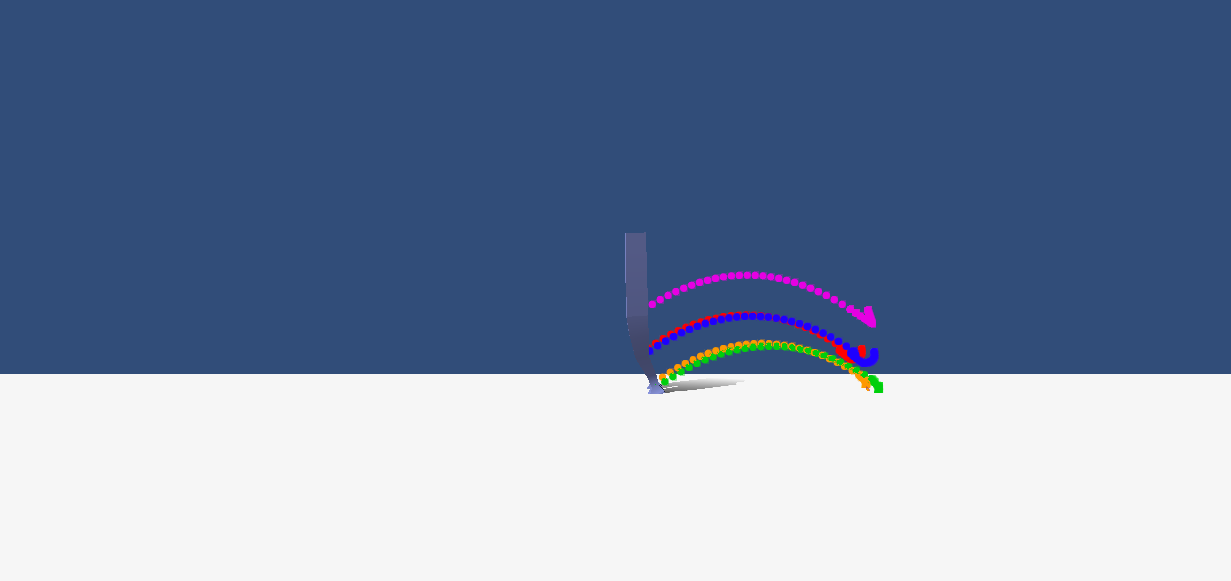
\includegraphics[width=\textwidth]{images/trails/trail-side.png}
	\caption[Marker trail visualization of motion]{An example of the markers tracking joints.  With a high sample rate, a curve forms trailing along the path of the joint.  Markers were placed at a rate of 10 per second of simulation time.}
	\label{fig:marker_trails}
\end{figure}

Markers were implemented as camera-facing ``billboard'' planes with a texture that were spawned with a user-specified frequency, following an arbitrary joint of the character.  Each frame the orientation of the planes adjusts such that it faces the main active camera, allowing very little geometry to be used to produce an always visible visual to be placed in the scene.  I used one of these for each joint in the legs as well as one for the pelvis in order to track the paths of the joints.  This visualization was an interesting one to view, and gave a similar effect to motion sculptures, but was very difficult to understand without a reference to know which color of marker corresponded to which joint.  Even with knowledge of which joint followed which trail of markers, the visualization was difficult to understand, though it gave a good overview of the whole motion.  These marker trails are shown in Figure \ref{fig:marker_trails}.

\begin{figure}[ht]
	\centering
	\begin{subfigure}[b]{0.49\textwidth}
		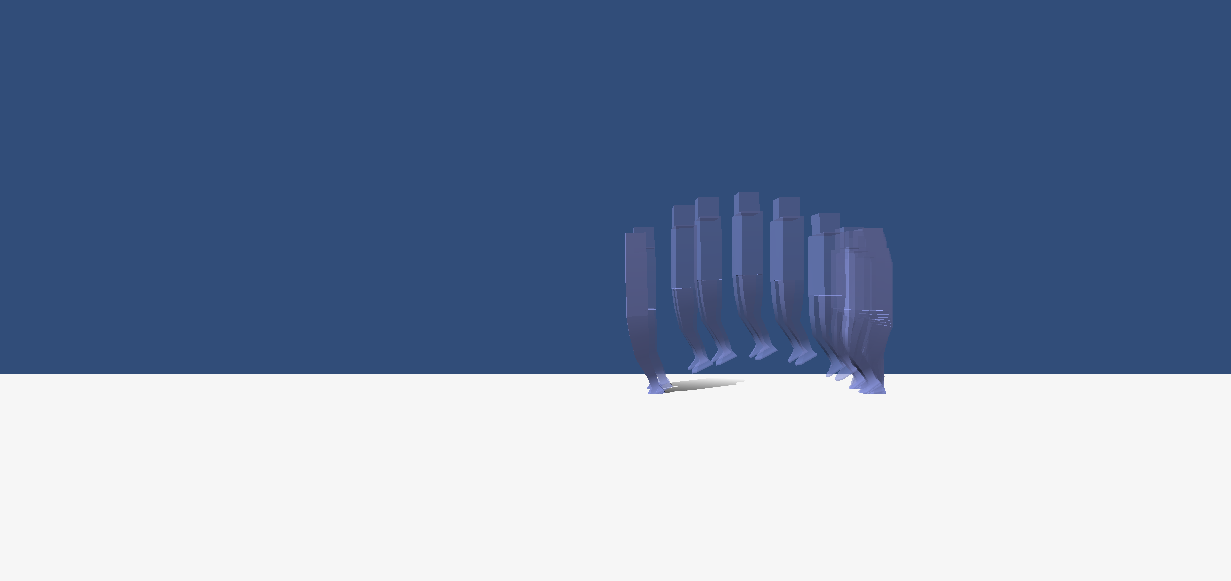
\includegraphics[width=\textwidth]{images/ghosts/side-sparse.png}
	\end{subfigure}
	\begin{subfigure}[b]{0.49\textwidth}
		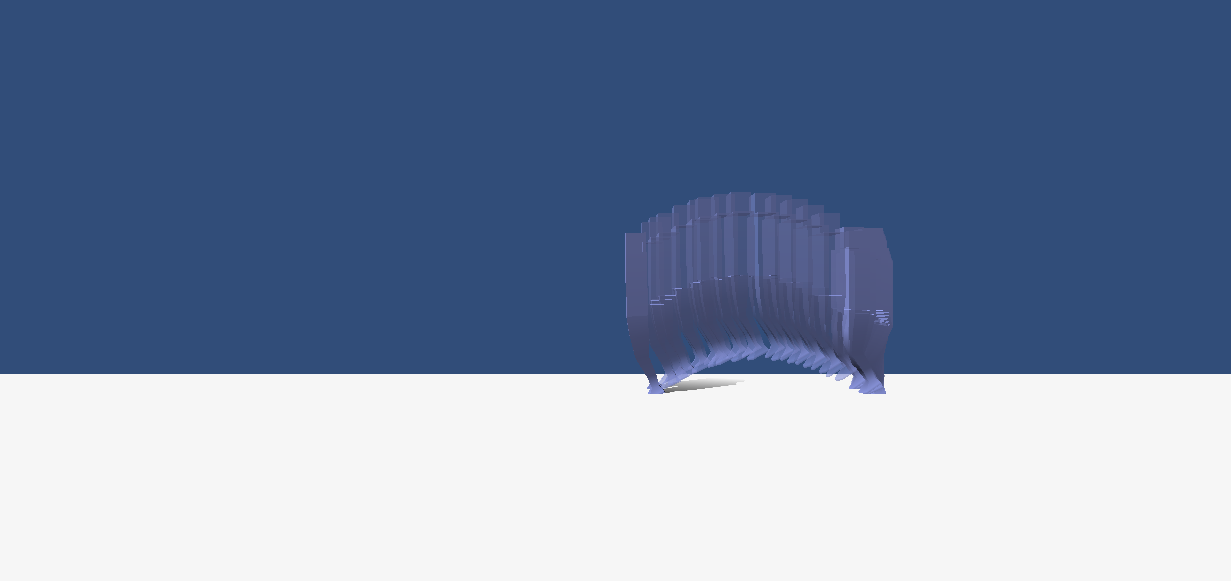
\includegraphics[width=\textwidth]{images/ghosts/side-dense.png}
	\end{subfigure}
	\caption[Ghost image visualization]{Pictured above are examples of a ghost image visualization achieved by placing copies of the character model at a rate of 1 per 0.5s (pictured left) and 1 per 0.2s (pictured right).}
	\label{fig:ghost_vis}
\end{figure}

I used a ghost image visualization as well in 2 ways: leaving copies of the character behind at a user defined rate and layering collected frame data.  In the first method, I make a copy of only the model and necessary skeleton components, leaving out the extra data such as mass, constraints, and muscles used in my simulation, and match the positions and rotations of each of its joints to the character at the current time.  The ghosts use a semi-transparent material to help differentiate between them and the model, as well as to provide some clarity as to each ghost's pose and combat the issues of occlusion.  Examples of this visualization are shown in Figure \ref{fig:ghost_vis}.

\begin{figure}[ht]
	\centering
	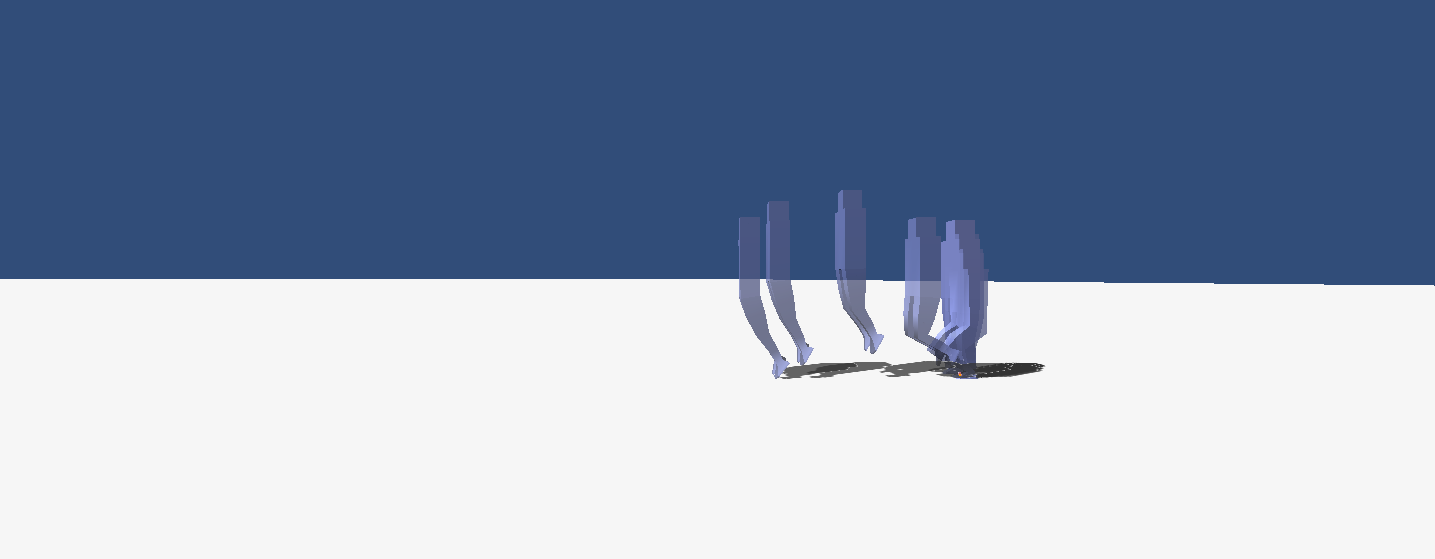
\includegraphics[width=\textwidth]{images/k200kvaryingcomposite.png}
	\caption[Composite frame visualization]{An example of the composited frames visualization, in which several frames of the animation are layered on top of each other, and matte painted to produce a combined image with all frames superimposed.}
	\label{fig:composite_vis}
\end{figure}

An alternate method of forming the ghost image visualization was to layer numerous collected frames in an image editing program.  This method was very work intensive, requiring each layer to be matte painted by hand.  Algorithms and techniques in image processing and computer vision for automating this process, but for my purposes it was necessary to manually select the desired region in each image that should be visible in the final combined image.  To reduce the negative effects of occlusion, layers above the first were given an opacity of $75\%$.  Though work intensive, this produced an excellent visual for still media to show the path of the entire motion, but was a poor visual in many cases for showing detail of the movement as images often occlude each other.  Examples of this visualization are shown in Figure \ref{fig:composite_vis} and in Figure \ref{fig:complex_scene}.  As a compliment to this visual, I used animation strips, in which the frames were simply presented adjacent to each other in order from left to right.  These strips are also found in the data tables presented in Section \ref{section:image_results} and in Figure \ref{fig:complex_scene}.

\section{Debugging Visualizations and Controls}
\label{section:debug_control_vis}

For debugging visuals, I used a feature in \unity{} called Gizmos \footnote{http://docs.unity3d.com/ScriptReference/Gizmos.html [Accessed: August 10, 2015]}, which allowed debug drawing of primitive shapes.  I used small spheres of various colors to show sample positions, target positions for the IK solver, corners of the supporting polygon, and the position of the center of mass.  Rays were used to visualize velocity, acceleration, distance to the destination, and value of the samples.  A screenshot of my Gizmos active for an energy based simulation are shown in Figure \ref{fig:gizmo_vis}.

\begin{figure}[ht]
	\centering
	\begin{subfigure}[b]{0.49\textwidth}
		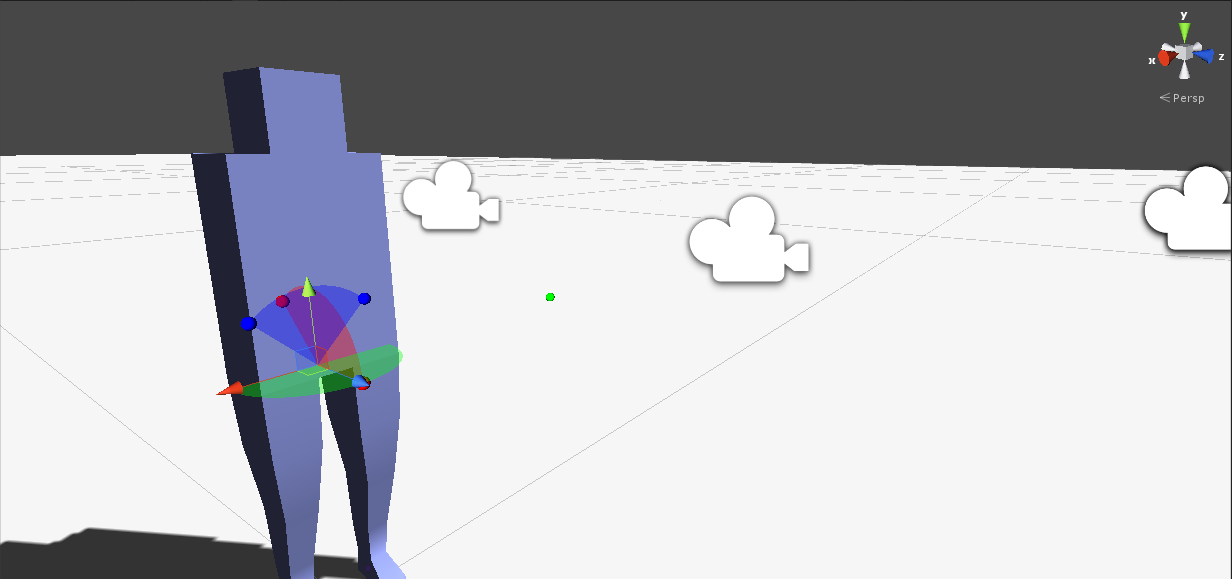
\includegraphics[width=\textwidth]{images/handles1.png}
	\end{subfigure}
	\begin{subfigure}[b]{0.49\textwidth}
		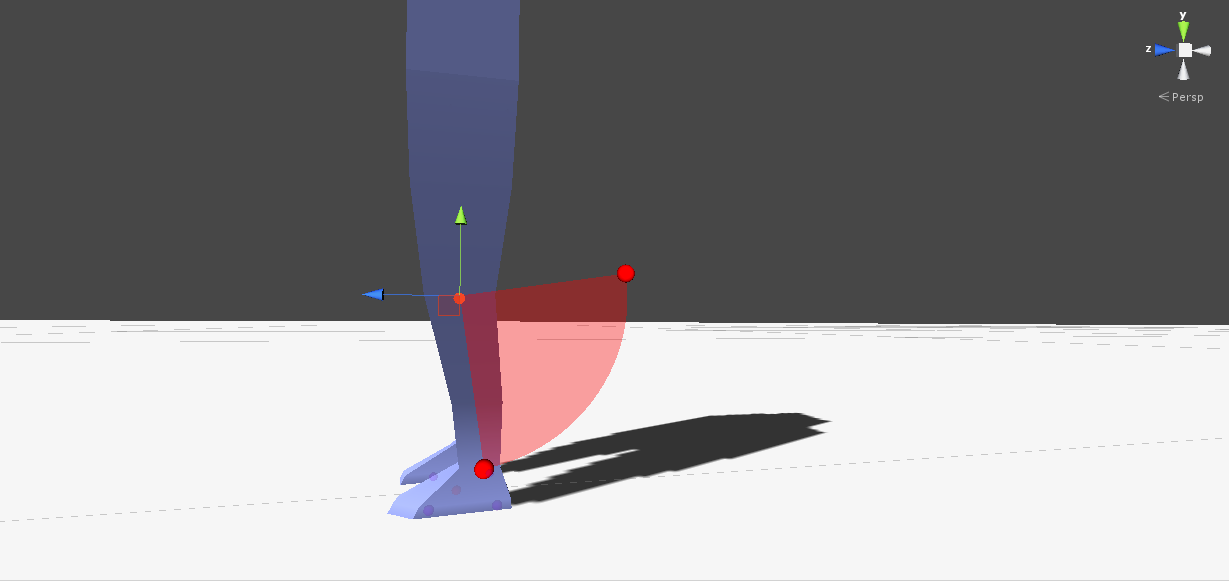
\includegraphics[width=\textwidth]{images/handles2.png}
	\end{subfigure}
	\caption[Screenshot of Handles used for setting and visualizing joint constraints in \unity{}]{Screenshots of Handles, a tool in \unity{} which allows the user to create custom UI elements in the editor for changing a value in the game or simulation.  In this case, the Handles affect the minimum and maximum rotation for the joints.  Handles are only visible when the corresponding object is selected by the user, reducing clutter.  All three Handles are shown in the left image, allowing the user to set the constraints for pitch (red), yaw (green), and roll (blue) as the pelvis is set to allow rotations about all three axes.  At right, I show the Handle for adjusting the constraints of the left knee, which is only able to rotate about the x-axis (pitch).}
	\label{fig:handle_vis}
\end{figure}

Similar to the Gizmos, I utilized a feature called Handles \footnote{http://docs.unity3d.com/ScriptReference/Handles.html [Accessed August 13, 2015]} to ease setting and visualization of the joint constraints on the skeleton.  Unlike a Gizmo, a Handle can be manipulated by the user to affect values in the simulation before run time.  As shown in Figure \ref{fig:handle_vis}, three handles were used to adjust pitch, yaw, and roll, color coded as red, green, and blue.  Colors were chosen to correspond to the colors of the reference axes placed in the scene to aid the user, showing the red, green, and blue handles as limiting rotation about the x, y, and z axes respectively.

\begin{figure}[ht]
	\centering
	\begin{subfigure}[b]{0.49\textwidth}
		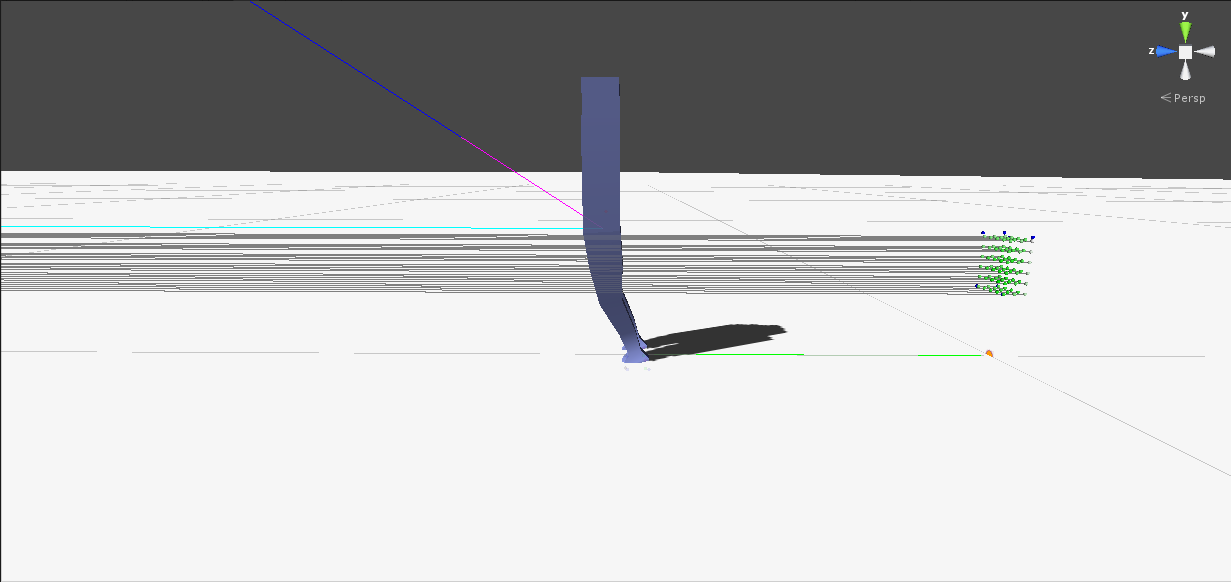
\includegraphics[width=\textwidth]{images/gizmos1.png}
	\end{subfigure}
	\begin{subfigure}[b]{0.49\textwidth}
		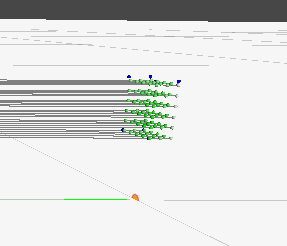
\includegraphics[width=\textwidth]{images/gizmos2.png}
	\end{subfigure}
	\par\medskip
	\begin{subfigure}[b]{0.49\textwidth}
		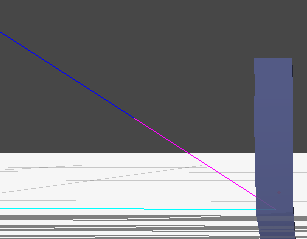
\includegraphics[width=\textwidth]{images/gizmos3.png}
	\end{subfigure}
	\begin{subfigure}[b]{0.49\textwidth}
		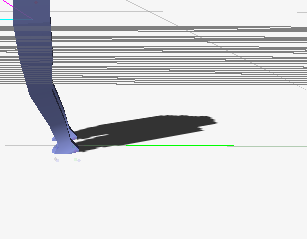
\includegraphics[width=\textwidth]{images/gizmos4.png}
	\end{subfigure}
	\caption[Screenshot of Gizmos used for debug visualizations in \unity{}]{Screenshots of Gizmos in the \unity{} Editor.  The green points illustrate the sample field taken at the beginning of the jump, while the gray lines show the energy measured at this sample.  The rays beginning at the player's pelvis show the magnitude and direction of the acceleration (magenta) and velocity (blue) of the character.  The green line at the player's feet shows the displacement from the start position to the destination, and the cyan line starting at the player's pelvis shows the calculated kinetic energy.  At right, a closer view of the samples is shown to show the blue dots which outline the balanced region which the samples were restricted to.  The character is distanced from these samples as the Gizmos are drawn at the character's start position, and the character in this scene has completed its jump and is at the destination position.  The orange particle is a marker placed at the start position.}
	\label{fig:gizmo_vis}
\end{figure}

\section{Discussion}
\label{section:vis_discussion}
The hope for the visualizations was to provide simple, at-a-glance diagnostics that would show an animation's strengths and shortcomings.  Tracking individual joints with markers provided surprisingly little information, though I had hoped it would provide a simplified way of looking at the overall motion of the character, eliminating unnecessary visuals of the character model and providing information purely about the skeleton.  While less useful than I had hoped, the trails following the joints did provide information about the general path of the character, though detail was often obscured by overlapping portions of the trail. One such case was where the character's foot was becoming trapped in the ground and ended up twisting in place, instead of remaining stationary as a support.  The twisting trail around the foot joint provided a simple visual that there was movement where there should not be.  This visualization also indicated that the information provided by the character model is necessary to understanding the animation of the character, leading to the ghost image visualization.

The ghost image visualization provided similar information, but kept the character model.   Due to the regular sampling of the character's position, this visualization was good for finding temporal issues, where the character spent too great or too small a time in different portions of the jump.  One such instance was that the character had an issue where the inverse kinematic solver could not keep up with the rate at which the character moved when performing the windup animation for a ``superman'' jump, in which the muscles were tuned such that the character could jump to the top of a 200m block.  The motions occurred too quickly due to the large values involved, necessitating a finer timestep so that the simulation would not overshoot.  This visualization showed the back-and-forth adjustments occurring due to the simulation constantly passing the target pose by over-adjusting.

The Gizmo visuals were used out of necessity.  The dots were inserted in order to visualize the samples and the values that each produced, as the output animations for early iterations were very far from expected motions and the animation itself provided very little information about the target or calculated values.  These visualizations helped to find mathematical errors in the torque-based simulation, as well as leading to the abandonment of the torque-based simulation in favor of the energy-based simulation when the values of the torque-based simulation remained very far from expected, but the energy-based simulation produced similar values to those expected.  The gizmos were also used to visualize the balance of the character, showing center of mass and the supporting polygon.

Handles were used as a utility, as setting the angle constraints on the joints of the character was a long and difficult process, with very little to indicate if the range was ``realistic'' or ``expected.'' The angles in \unity{} are not always as expected, since a rest angle of the joint may be $0^\circ$, while biologically the rest angle may be defined as $180^\circ$.  Handles provided a way to have not only a visual representation of the constraints on the joints, but also a more intuitive method of entering them.  Instead of typing in the numbers in the \unity{} Inspector, the Handles may be dragged to modify the values.  Creating Handles for the specification of muscles would likely make the process of setting up the skeleton much easier and more intuitive for animators, and is of high priority for future iterations of this system.

\section{Summary}
In this chapter I discussed some difficulties in visualizing animations in both animated and non-animated settings.  I presented some sources of inspiration and discussed the different methods I used to visualize data for presentation, analysis, and debugging.  Methods I used for analysis and presentation included trails of markers, ghost images created by duplicating the player model in the scene, layering frames to create a single image, and animation strips.  My debugging visualizations took advantage of \unity{} utilities, using Gizmos and Handles to allow the user to see information about the simulation, as well as to more easily adjust constraints on the skeleton.
\label{section:vis_summary}
